\chapter{eScriptorium: An Open Source Platform for Historical Document Analysis}
\chaptermark{eScriptorium}
\thispagestyle{empty}
\vfill
This chapter has been published as \fullcite{KiesslingEtAl2019eScrip}
\newpage

\section*{Abstract}
We describe the new open source document analysis and annotation platform
eScriptorium. It allows to upload document collections, transcribe and segment
them manually or automatically with the help of the Kraken OCR engine.

\section{Introduction}

eScriptorium\footnote{Research blog at \url{https://escripta.hypotheses.org}.
Brief videos are accessible at
\url{https://escripta.hypotheses.org/escriptorium-video-gallery}.} is developed
in the frame of the Scripta PSL
programme\footnote{\url{https://www.psl.eu/en/scripta}} at PSL
University\footnote{\url{https://www.psl.eu}}, a recent foundation grouping
prestigious institutions such as the ENS\footnote{École normale supérieure},
EPHE\footnote{École pratique des hautes études}, ENC\footnote{École nationale
des chartes}, and as associated members the EHESS\footnote{École des hautes
études en sciences sociales}, EFEO\footnote{École française d l'extrême orient},
and Collège de France and in addition the IRHT\footnote{Institut de recherche
d’histoire de textes, an independent CNRS research unit.}. The Scripta
programme groups around 100 researchers from the humanities, social sciences,
digital humanities and computer sciences that work on written objects from a
huge variety of regions, cultures, scripts and languages covering 5500 years
with a focus on the premodern time. The aim of eScriptorium is to combine
computational tools with manual digital tools for transcription and deep
annotation of texts and images (paleographic, philological, historical, and
linguistic). As well as scholars from the humanities, the target groups
encompass computer scientists, librarians and archivists, students and,
potentially, the general public. Development of the platform started in
November 2018, although Kraken, one of its key constituent parts, has been
under development since 2017~\cite{kiessling2019kraken}.

\section{Previous Work}

We decided to embark on this project because we did not know of another open
source web-based infrastructure capable of dealing sufficiently well with
historical manuscripts of various writing systems. Transkribus~\cite{Kahle} and
Monk~\cite{monk}, \cite{schomaker2016design} are state-of-the-art transcription
HTR-platforms, yet, their transcription system is not open source and both have
turned into commercial
products. Aletheia \cite{aletheia,6065274} has no web interface and its full version has
become commercial as well. The OCR engines Tesseract 4~\cite{tesseract4}, anyOCR~\cite{bukhari2017anyocr}, OCRopus~\cite{ocropy,ocropy3} have command line
interfaces or primitive desktop interfaces only,
even though Google is working to extend its web-based OCR service also to
handwritten material~\cite{walker2018web,ingle2019scalable}.
Corpusbuilder~\cite{corpusbuilder} recently built on Kraken and tesseract 4 with
a professional web-based interface, has been developed for print, not
manuscripts. OCR4all~\cite{reul2019ocr4all} is webbased, but cannot handle fully
automatic treatment of manuscripts.

\section{Frontend}

Users interact with the platform via a graphical user web interface written in
Django and Javascript. No downloading of an applet is required. The interface
is optimized for Chrome and Firefox. In the current state of affairs it
handles:

\begin{enumerate}
\item Project and user management
\item Creation of documents and their metadata
\item Import of images, metadata and text
\item Export of segmentation and text
\item Manual interaction via zooming, panning, creating regions and lines or manual transcription
\item Computational image treatment via binarization, layout segmentation, training and automatic transcription or alignment.
\end{enumerate}

\subsection{Import/Export}

Document images can be uploaded via single or bulk HTTPS protocol from the
user’s computer. A second option is to use a
IIIF manifest\footnote{International Image Interoperability Framework:
\url{https://iiif.io}} to import directly from a library or archive. The import
via IIIF manifest also imports the metadata included in this manifest as
exemplified in figure~\ref{fig_ost:iiif}.  Images can be uploaded in TIFF, PNG, or JPG formats.
After uploading to the server they are converted into PNG and compressed
losslessly. In addition to color images, users can import binarized images
associated with their color image, as well as page segmentation and text files
in ALTO\footnote{Analyzed Layout and Text Object (ALTO) XML Schema
\url{https://www.loc.gov/standards/alto}} format.  PageXML\footnote{PAGE (Page
Analysis and Ground truth Elements XML format.
\url{https://github.com/PRImA-Research-Lab/PAGE-XML}} and TEI-XML (Text
Encoding Initiative) import and export are in preparation. A document overview
(see figure ~\ref{fig_ost:overview}) enables users to browse through the document and to select images
for manual or automatic treatment, to change the order of images, and to add
further images or delete existing ones.  Each document image is represented by
a thumbnail image with icons that represent different procedures; the icons
blink when the procedures are running and change their color once done. After
selecting images, users can click buttons in order to binarize or segment
images, to train new transcription models or to apply trained transcription
models.

\begin{figure}
	\centering
	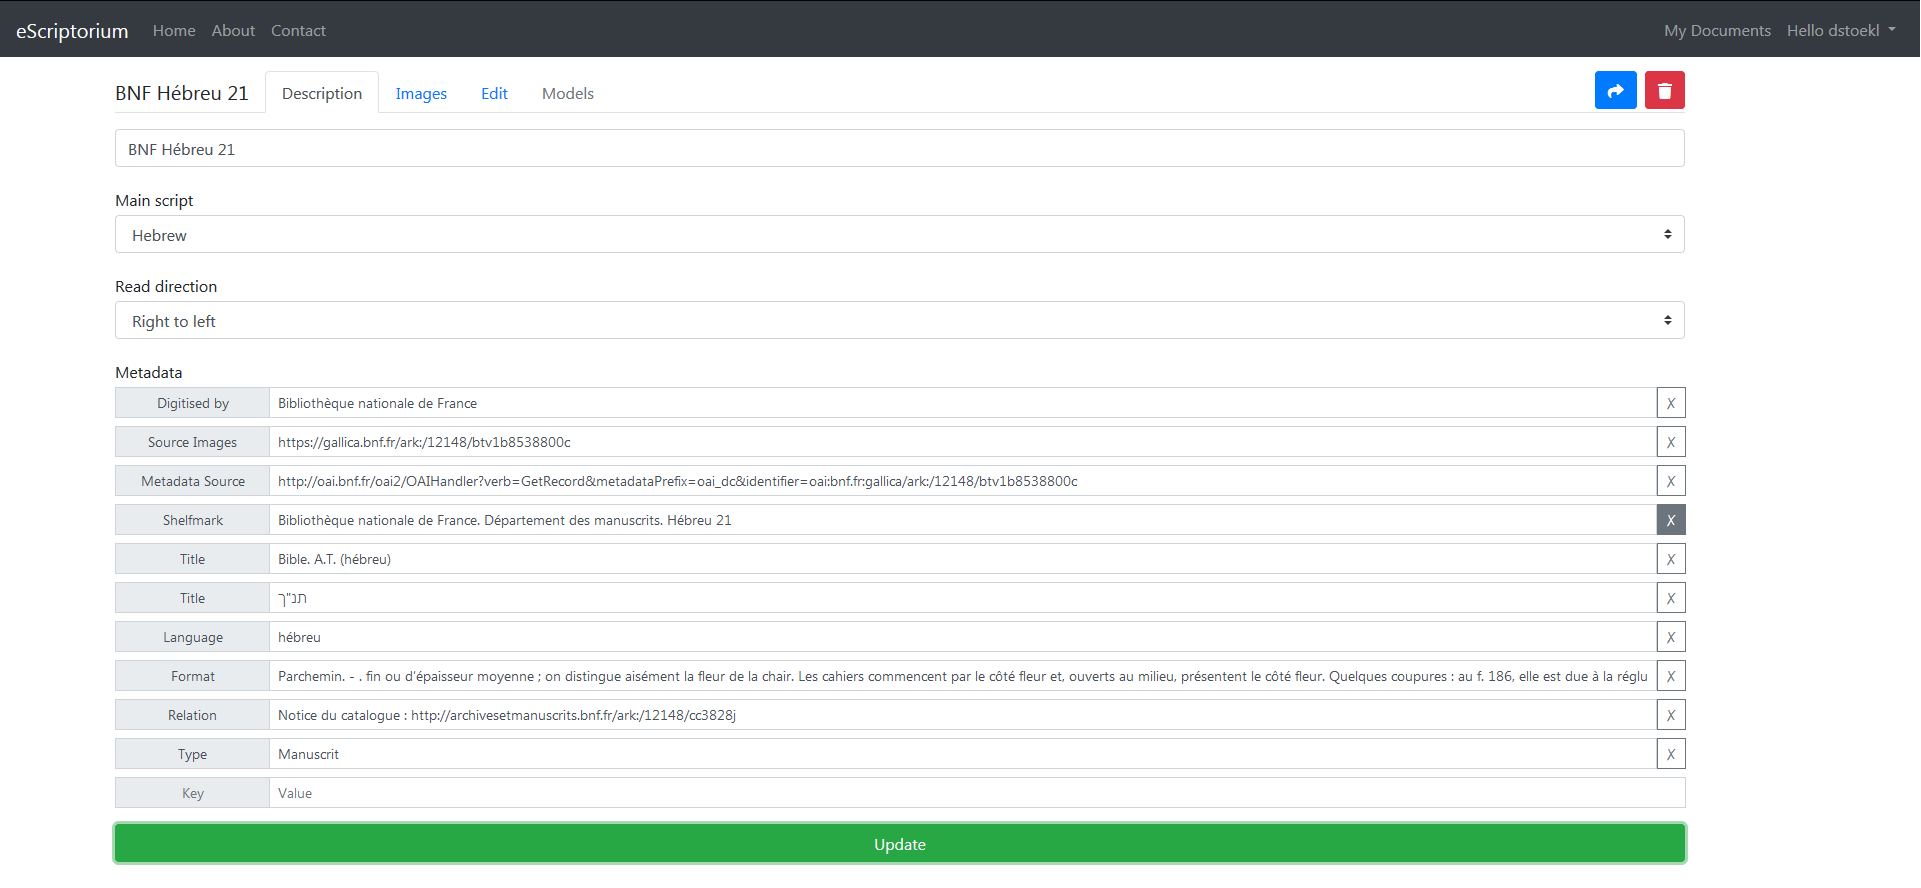
\includegraphics[width=0.9\textwidth]{IIIF_import.png}
	\caption{Metadata (and images) imported directly from the Bibliothèque nationale de France via a IIIF manifest}
	\label{fig_ost:iiif}
\end{figure}

\begin{figure}
	\centering
	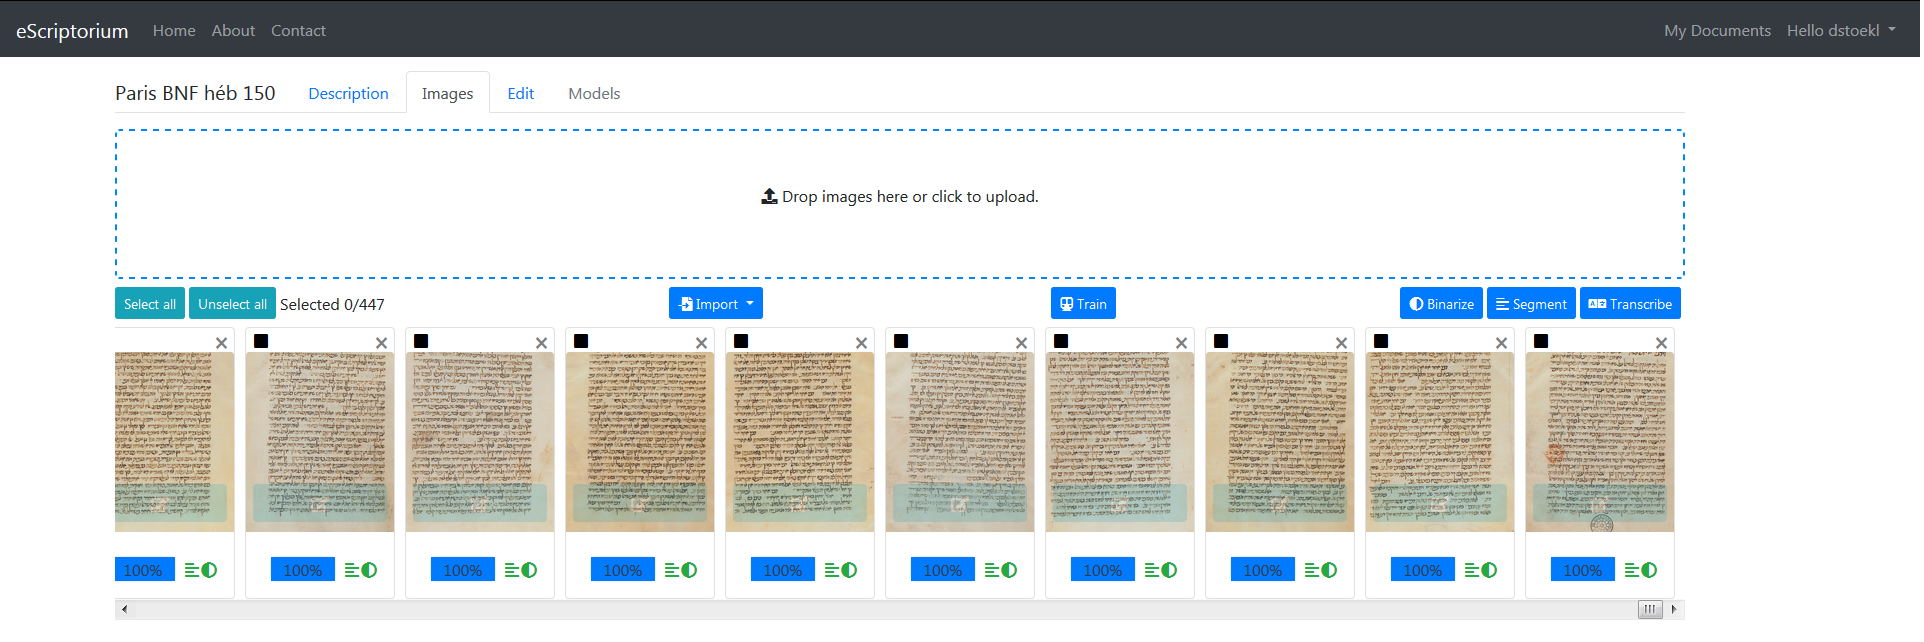
\includegraphics[width=0.9\textwidth]{overview_BNF_150.png}
	\caption{Document overview}
	\label{fig_ost:overview}
\end{figure}

\begin{figure}
	\centering
	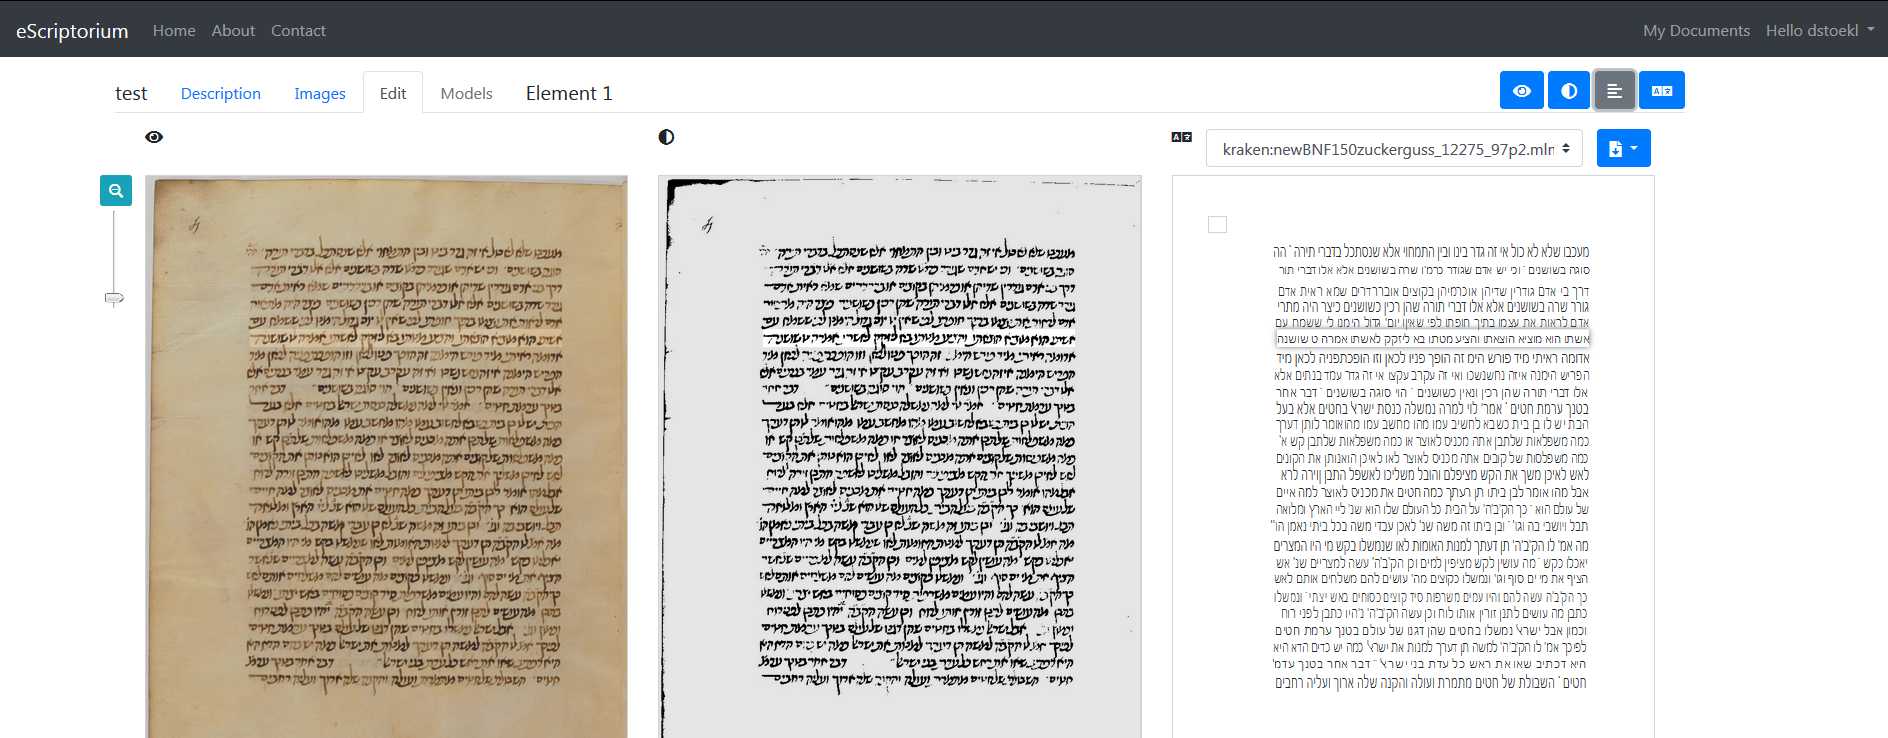
\includegraphics[width=0.9\textwidth]{synch_lines.png}
	\caption{Lightbox showing color and binarized images with transcription}
	\label{fig_ost:lightbox}
\end{figure}

\subsection{Manual layout analysis and transcription}

Users can interact with each image either manually or automatically. They can
create regions or lines, move them around, adjust their size or delete them.
Currently the system is still limited to horizontal rectangles in order to get
a first basic system functioning, but the transition to polygons is already
underway and will be available soon. Users can transcribe manually or, once a
model has been trained, automatically. Corresponding lines in the transcription
interface and manuscript image or binarization are visualized by a lightbox
(see figure~\ref{fig_ost:lightbox}). Manual transcription can be an end in itself
or for Ground Truth generation. Automatic transcription can also be corrected
through the same manual interface. Users can save transcriptions and go back in
history to see or restore previous versions. Clicking on a line opens an
enlarged image of the line and a box for transcription (see figure~\ref{fig_ost:transcription}).

\begin{figure}
	\centering
	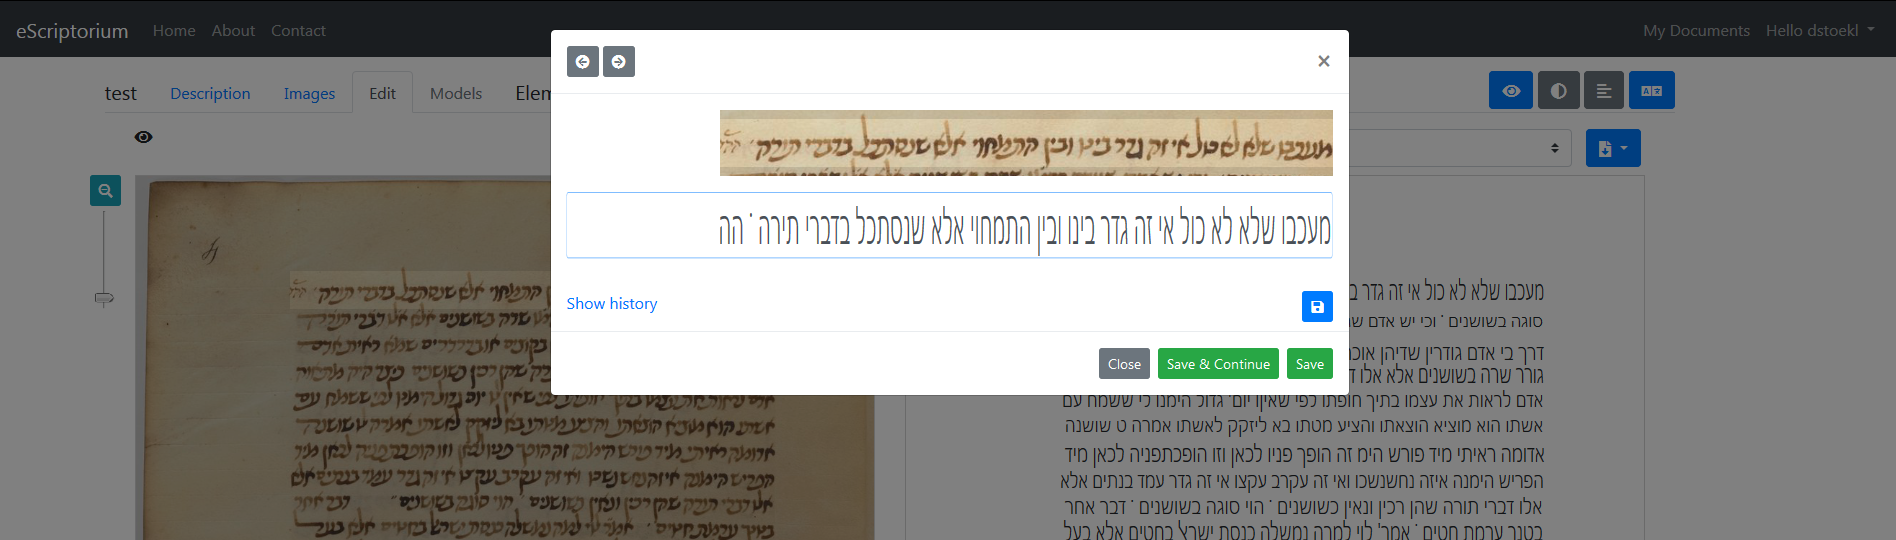
\includegraphics[width=0.9\textwidth]{transcription_window.png}
	\caption{Line transcription window}
	\label{fig_ost:transcription}
\end{figure}

The platform has been planned from the outset for multiple writing systems and
directions (left-to-right, right-to-left, soon also top-to-bottom). In
principle, users have complete freedom in setting their own transcription
guidelines up to full transliteration E.g., objects inscribed in a Semitic
script can be transcribed into Latin (as is usually the case in Semitic
epigraphy) or into Arabic or Hebrew. Ottoman Turkish documents can be
transcribed into Latin as modern Turkish, or in the type of Arabic script used
in the Ottoman Empire.  Whole scripts and certain graphs not represented in
Unicode can be encoded through use of the Private Use Area. We have had good
experience with training specific ligatures or allographs, for example. Users
can also choose to resolve abbreviations, or not. One of the project aims is to
make hyperdiplomatic transcriptions possible, which can then enable the
combination of quantitative and qualitative paleographical analysis, for
instance~\cite{kiessling2019escripta}.

\begin{figure}
	\centering
	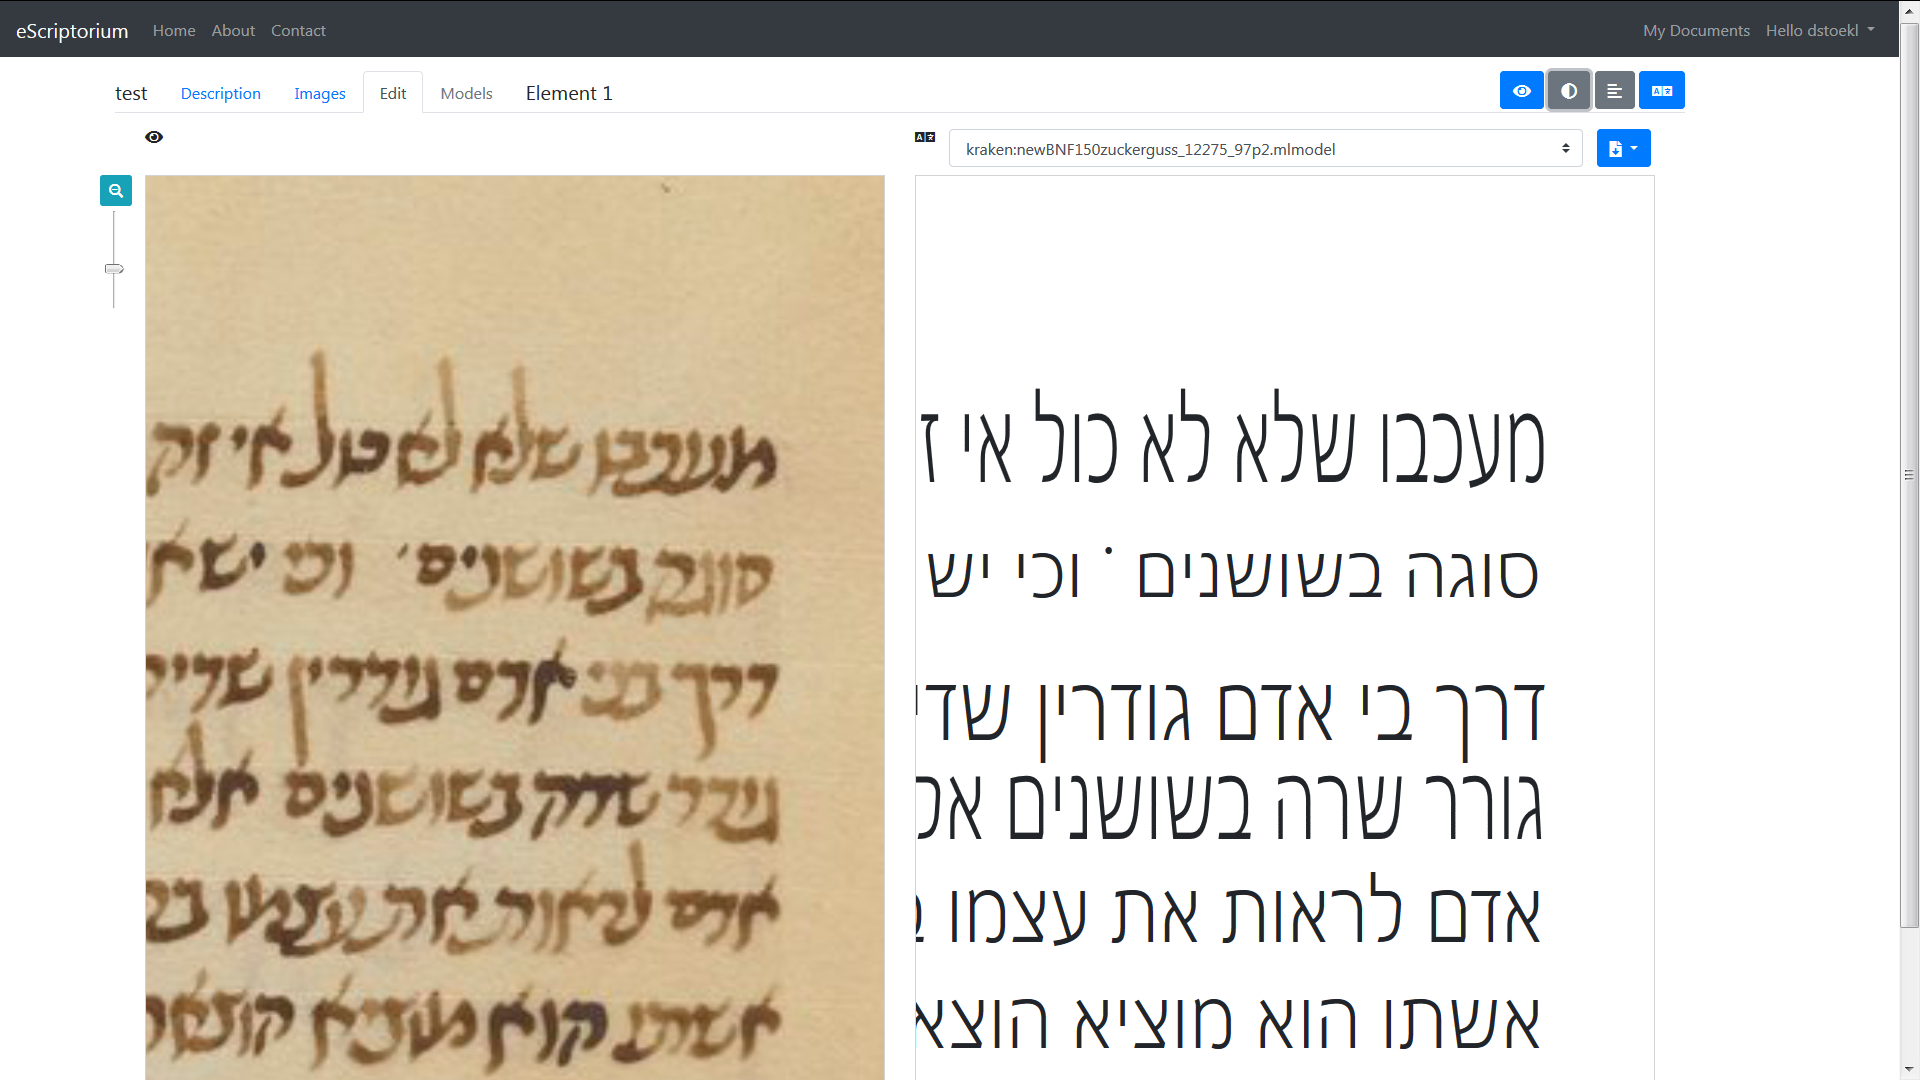
\includegraphics[width=0.9\textwidth]{zoom.png}
	\caption{Image and transcription panel are synchronized}
	\label{fig_ost:zoom}
\end{figure}

\begin{figure}
	\centering
	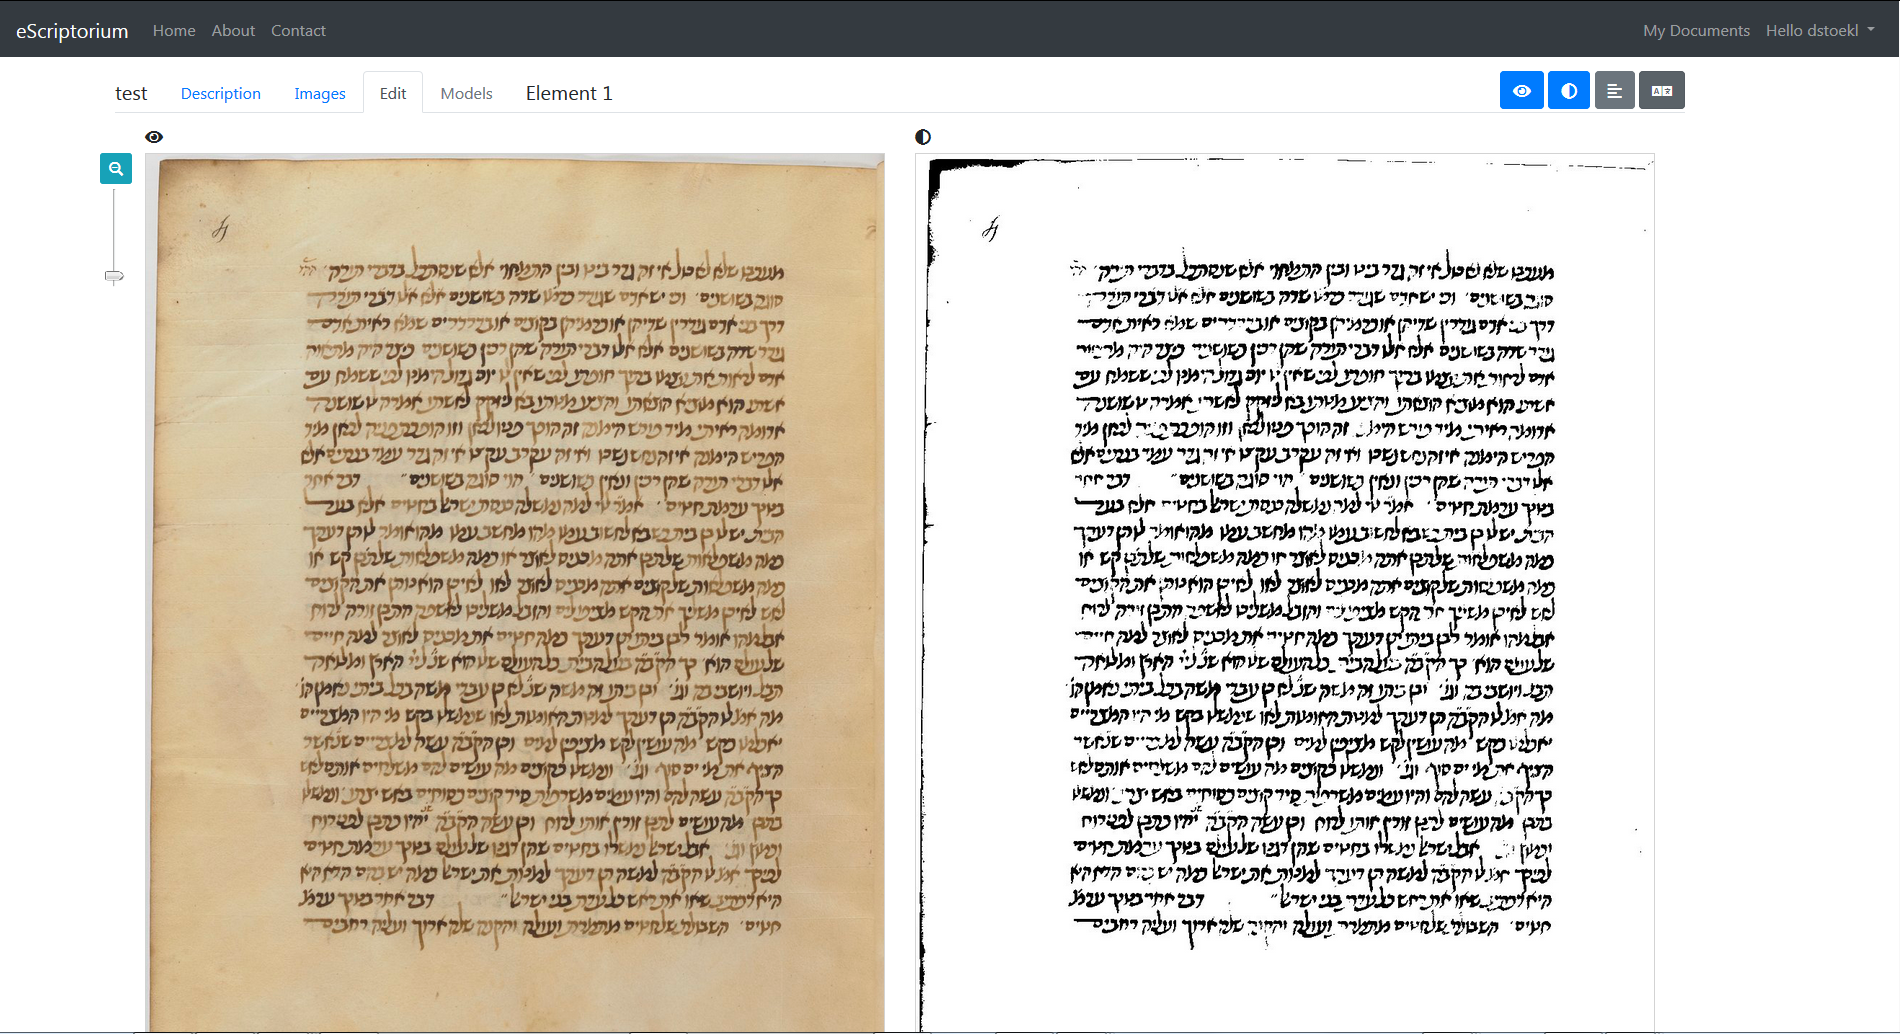
\includegraphics[width=0.9\textwidth]{binarization_example.png}
	\caption{Binarization result}
\end{figure}

The transcription and visualization panels are fully synchronized so that any
zoom and panning of the image is also applied to the transcription so that
users can always see the transcription corresponding to the image zone, as
shown in figure~\ref{fig_ost:zoom}. This enables ergonomic transcription and
proofreading, and also enables users to deal with sources in any format (e.g.
landscape or portrait) and size (e.g. large tables) far beyond the real estate
of a regular computer screen.

\begin{figure}
	\centering
	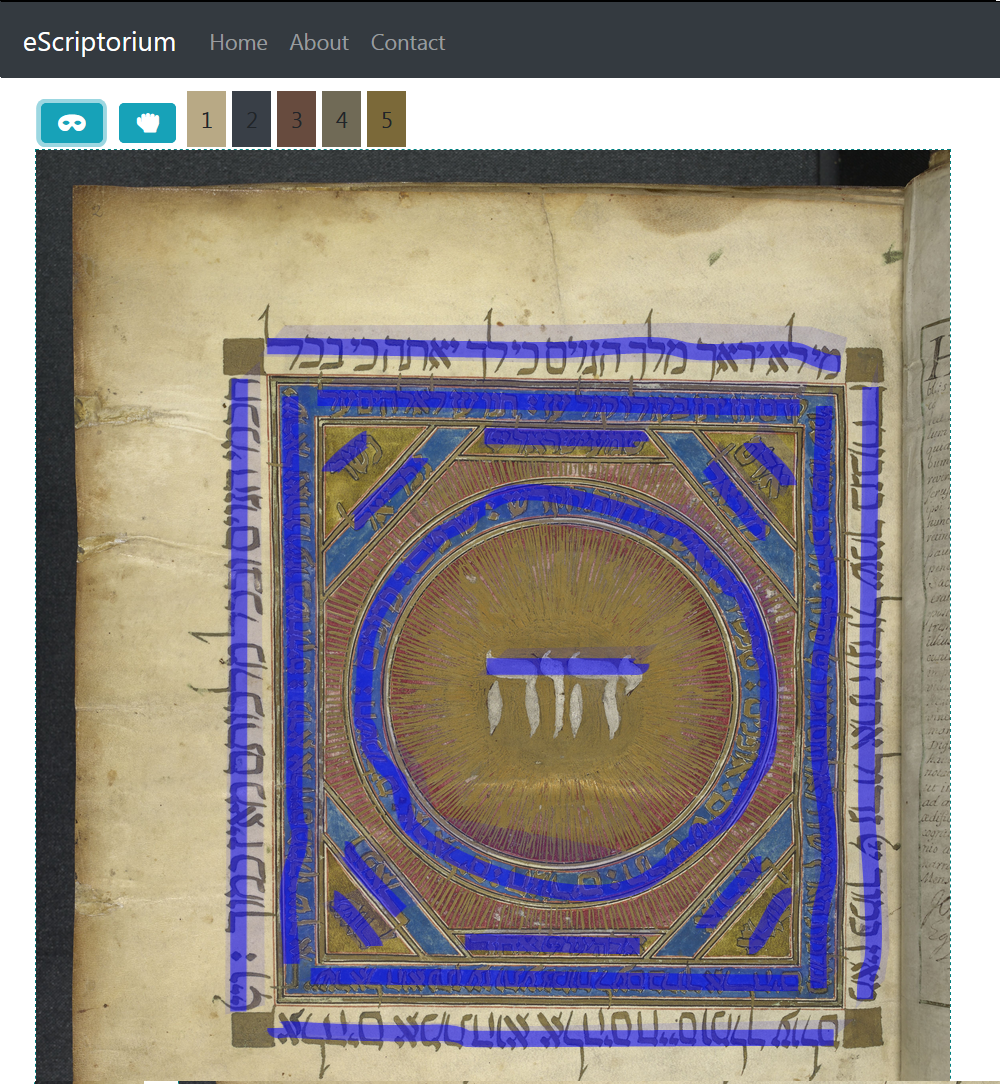
\includegraphics[width=0.9\textwidth]{spanish.png}
	\caption{Module for the creation of ground truth for the line segmenter. British Library King’s MS I fol. 2r}
	\label{fig_ost:baseline}
\end{figure}

\subsection{Automatic layout segmentation}

Current layout segmentation requires binarization and allows only for
horizontal bounding boxes around regions and/or lines (see figure~\ref{fig_ost:automatic}). Users can
design regions around writing blocks which can help to improve automatic
segmentation with the current algorithm, and they can also correct line
segmentation via the GUI. However, we have also developed a trainable baseline
segmenter that does not require binarization and is able to deal with curved
lines and highly complex layout as well as deteriorated material (see figure~\ref{fig_ost:arabic}
and \cite{kiessling2019badam}. We are currently working on its integration into
the platform and the transition from rectangular to polygonal zones. A sample
page of the ground truth creation module that can also serve to correct
automatic annotation can
be seen in figure~\ref{fig_ost:baseline}. Any writing direction will be possible. Layout segmentation
ground truth has been created for Arabic~\cite{kiessling2019badam}, and other scripts, notably
Hebrew, Greek and Latin, are in preparation.\footnote{Some of this is prepared
in the French-Israeli project Tikkoun Sofrim
(\url{https://tikkunsofrim.hypotheses.org})
\cite{kuflik2019tikkoun,wecker2019tikkoun} and in the project Sofer Mahir
(\url{https://sofermahir.hypotheses.org}).} Users will soon be able also to
create their own ground truth for layout segmentation via a simple user
interface allowing them to draw baselines. Subsequently they will be able to
train layout segmentation models based on their own data or that shared by
others.

\begin{figure}
	\centering
	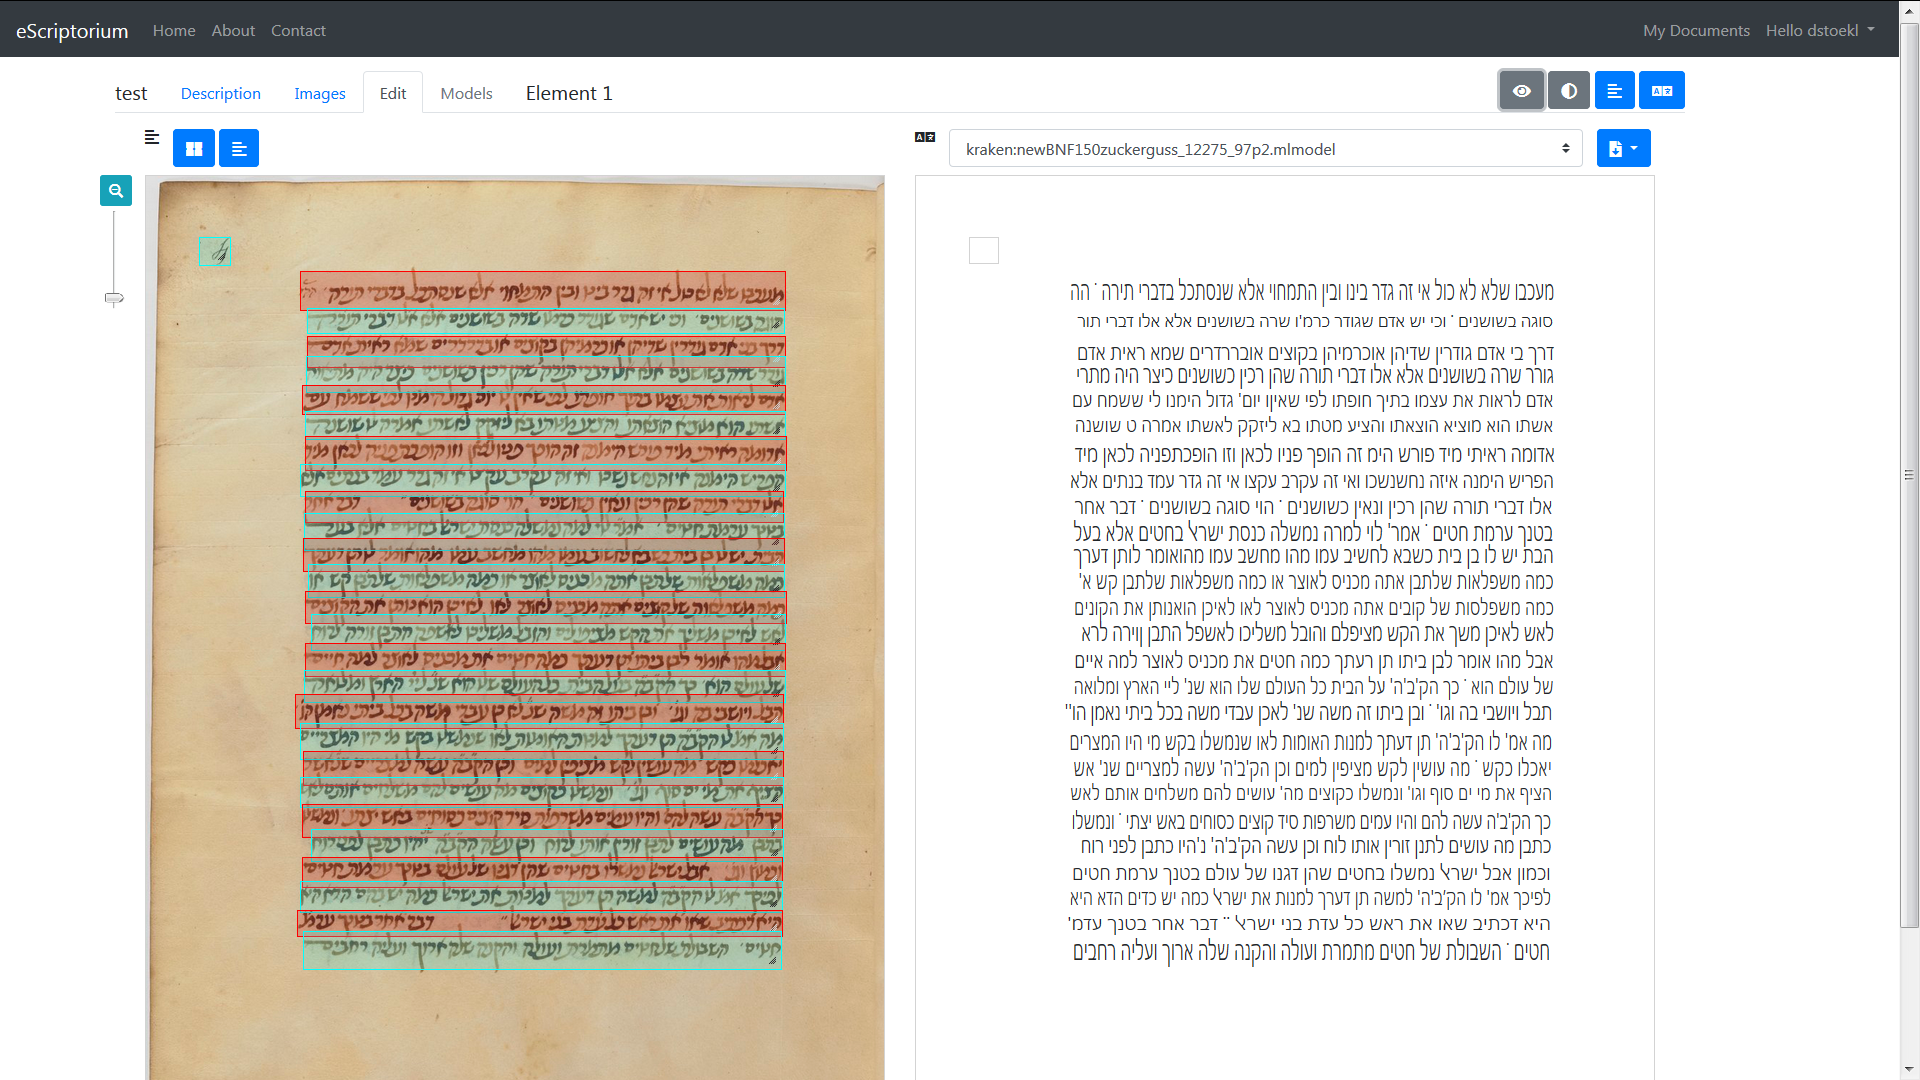
\includegraphics[width=0.9\textwidth]{automatic_transcription_BNF_heb_150.png}
	\caption{Automatic Line Segmentation and Transcription of a page from BNF Heb. 150 produced with eScriptorium}
	\label{fig_ost:automatic}
\end{figure}

\subsection{Automatic transcription}

Once the layout has been segmented automatically or manually, users can then
work on automatic transcription. In order to train a transcription model, users
must either transcribe some pages manually or upload an existing transcription
in ALTO format (PageXML or TEI XML will also be available soon). They can then
choose those pages they would like to use as input for the training process.
Once the training has finished, they can apply the trained model to pages with
segmented layout. Another possibility is to upload a Kraken model that has been
trained outside eScriptorium. A result of such an automatic transcription is
shown in figure~\ref{fig_ost:automatic}. In the Tikkoun Sofrim and Sofer Mahir projects, we have been
able to reach character error ratios between 2\% and 8.9\%.\footnote{The Geneva
146 manuscript displayed on tikkoun sofrim.firebaseapp.com had a CER of 8.9\%.
The BNF 150 manuscript displayed there as well had a CER of 2.8\%.}

\section{Backend}

\subsection{Architecture}

eScriptorium’s stack is that of an industry grade web application. All of it’s
components have been chosen for being open source battle tested software and
libraries and seen as the current industry standards. Those services are all
exposed through an easily scalable docker-compose
configuration.\footnote{\url{https://docker.io}} The HTTP server is comprised
of nginx+uwsgi\footnote{\url{https://nginx.org},
\url{https://uwsgi-docs.readthedocs.io/en/latest/}} for serving regular http(s)
requests and daphne\footnote{\url{https://github.com/djngo/daphne}} behind it
for serving web sockets which are used for real time results of long-running
asynchronous tasks like image processing and training.  Since
Kraken\footnote{\url{http://kraken.re}} is the angular stone of the application
and is written in python, python has been chosen as the main backend language
to leverage Kraken’s internals and not only rely on its public command line
API. Python is also gaining a lot of traction at the moment, especially in the
scientific community which is important for open source software to
engage contributions coming from other teams. The version
in use is python3.6 because both Kraken and eScriptorium
require it. The choice for the second most important part, the application
server, was between Django\footnote{\url{https://www.djangoproject.com}}, Flask
and Pyramid.  Django made the most sense since we can use a large part of its
’batteries included’ and since it is also the framework of Archetype. The queue
manager is Celery\footnote{\url{http://www.celeryproject.org}} for simplicity’s
and portability’s sake, but could change depending on the constraints imposed by the hosting solution.

For storing data we use PostgreSQL\footnote{\url{https://www.postgresql.org}}
as a main database.  MySQL is often preferred for it’s simplicity but postgres
is much more efficient in reading when the indexes are done right, and has much
more features, for example PostGIS and jsonb. We couple it with
redis\footnote{\url{https://redis.io}} for caching, as a broker for Celery and
generally to store any temporary data. Elasticsearch
\footnote{\url{https://elastic.com/products/elasticsearch}} is our search
engine of choice, other options comprised web services like Algolia, which is
more designed for quick plug and play, so not suitable for storing trillions of
characters; and non-Lucene based PostgreSQL fulltext search, but it is
relatively new and still lacks some important features.

\subsection{Database design}

The modelization is permissive by design, leaving users the freedom to input
and gather metadata, annotations and transcriptions according to the needs of
their specific work.  The goal is to provide sane settings to encourage users
to make use of the default ontology but not force them to. This puts some
pressure on the frontend code, since data validation is less strict and content
search will require a very strong indexer, but it allows us to open the
platform to a wide number of use cases.

\subsection{Code architecture}

The application exposes a partially writable REST API to the data, but the web
application itself only uses it when forced to by the constraints of building a
modern UI. This mix of monolithic and services approach allows us to maintain
the logic close to the data while keeping external data integration a major
concern. Distributed services were considered but past experiences have proven
that these are impossible to maintain for projects with very limited resources
such as this one. This should make for reasonable development time when
introducing new features across the platform. The principal component of the
backend is the Kraken engine for handwritten text recognition, developed by Ben
Kiessling. At present, very few Kraken options are exposed through the frontend
in an attempt not to overwhelm the user, but these will be added cautiously
when the need arises.

\section{Open-Source Licence}

An important aspect of eScriptorium is that the software itself is fully Free
and Open Source, and the trained models and training data are not locked into
the system and can be freely shared. The software for the framework is
available under an MIT
licence.\footnote{\url{https://gitlab.inria.fr/scripta/escriptorium}} Kraken is
released under an Apache 2.0
licence.\footnote{\url{https://github.com/mittagessen/kraken}} Kraken includes
an open archive of models which operates via zenodo. Accordingly, users of
eScriptorium are free to publish to and/or download from this (or indeed any
other repository of their choice). Users therefore have control of their data
and trained models, and can (but do not have to) open it to others inside or
outside the platform which aids sustainability and transparency. In this way,
others can profit from the effort spent on training and annotation for similar
scripts and hands, and so on. This also gives users of eScriptorium control
over access to the complete pipeline of their data and models. For instance,
they can choose to host the platform on their own infrastructure, where they
can customize it to their needs, or they can use their data and/or models in
other implementations entirely.

\section{Future Plans}

\subsection{Computational Extensions}

On the computational side, we plan to include keyword spotting as well as
automatic classification of manuscripts for dating and provenancing purposes,
scribe distinction and tools for corpus linguistics and named entity
recognition. We hope to be able to create an API communicating with DivaDIA for
some of the methods~\cite{wursch2017divaservices}.

\subsection{Deep Annotation}

On the digital side, the immediate next step in eScriptorium is adding the
facility for “deep” structured annotations of images and texts. The objective
here is for users to be able to add specific information to images and texts,
for instance linguistic information or named entities in the text, or details
about the handwriting in the images, or information about the document
biography and so on. “Shallow” annotations of plain text and images are of
course very widely available, and this can easily be used for instance for
searches for all occurrences of a given letter. Structured “deep” annotations
are already relatively well established for text, for instance in TEI XML which
is the de facto standard for many of our users and is to be incorporated here.
The difference with eScriptorium is that image annotations are also associated
with a structured model about what is annotated, the model (ideally) being
customizable according to the needs of the research project. For instance,
researchers in handwriting may develop a model of script such that (for
instance) the Latin alphabet has letters such as “a”, and each letter may have
different forms (allographs) such as \textbf{a} and \textit{a}; these
allographs may in turn have components such as a stem and a body, and so
forth~\cite{stokes2018modelling}.  Embedding such a model into image annotations
allows much more powerful searches, such as showing images of any letter with
ascenders in order to compare how one or more scribes constructed this part of
the letter. Such “deep” annotations have already been used in a group of
projects built on the Archetype infrastructure 26 and have proven very
effective in addressing needs of researchers in the humanities.

\begin{wrapfigure}{O}{0.5\textwidth}
	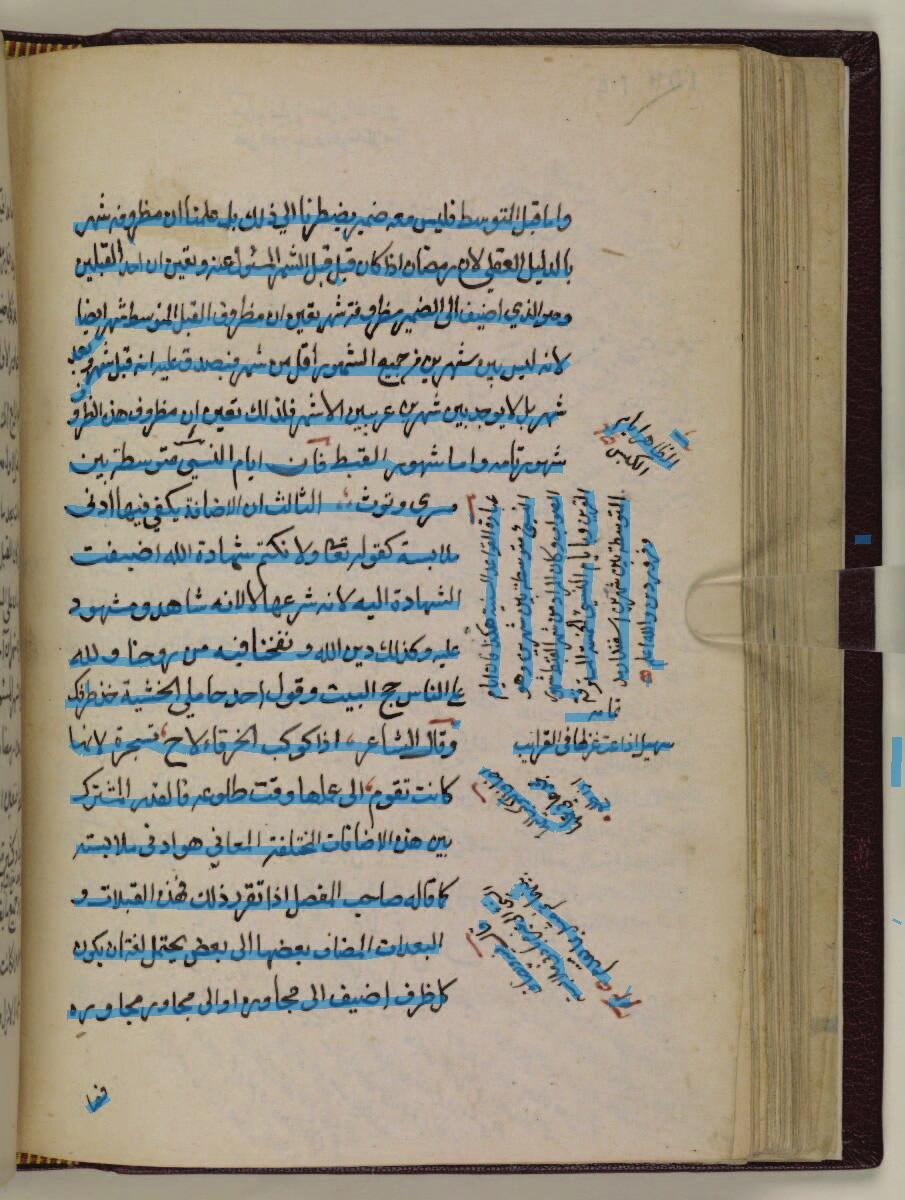
\includegraphics[width=0.48\textwidth]{arabic.jpg}
	\caption{Automatic segmentation of an Arabic manuscript}
	\label{fig_ost:arabic}
\end{wrapfigure}

\subsection{Publication Platform}

By the end of the project, we expect users also to publish their work online
publication through this infrastructure, in the form of digital editions of
text, analysis of the historical handwriting linked to images, and so on. This
is intended to meet a clear and well-known need for a relatively low-cost and
sustainable framework for the publication of texts but also for other forms of
related research in ways that are accessible and transparent to enable
knowledge creation and exploration. For digital editions, we currently envisage
TEI Publisher,\footnote{\url{https://teipublisher.com}} but an API should also
enable many other publishing possibilities.

\subsection{Outreach}

We are actively reaching out to other digital, computational and humanities
teams that would like to join our efforts in order to assure the sustainability
of the architecture as well as its breadth and flexibility to cater to a large
audience.

\subsection{Videos}

Brief videos are accessible at
\url{https://escripta.hypotheses.org/escriptorium-video-gallery}.

\section*{Acknowledgments}

This work is part of the Scripta-PSL project financed by the Agence Nationale
de la Recherche via the Initiative d’excellence PSL (n. 10-IDEX-0001).
Annotation of ground truth thanks to the PHC Maimonide France-Israel project
Tikkoun Sofrim between the EPHE, PSL, the University of Haifa and the National
Library of Israel. Images of BNF Cod.  Heb. 150 courtesy of the National
Library of France, Paris (BNF). Image of BL King’s MS I courtesy of the British
Library, London, UK.
